\documentclass[Lecture.tex]{subfiles}
\begin{document}
\section{Continuity}

\begin{frame}{Definition}
  \begin{defn}
    \begin{itemize}[<+->]
      \item
        We say a function, $f$, is {\it continuous at a point $a$ in the domain of $f$} if 
        $$\lim_{x \rightarrow a} f(x) = f(\lim_{x \rightarrow a}) = f(a).$$
      \item
        If $f$ is continuous at every point in an interval $(a,b)$, then we say that $f$ is {\it continuous on $(a,b)$}.
      \item
        If $f$ is continuous at every point in its domain, then we simply say that $f$ is {\it continuous}.
    \end{itemize}
  \end{defn}
\end{frame}

\begin{frame}
  Graphically, to say $f$ is continuous is to say that we can draw the graph without lifting our pen.
  \onslide<2->{
    Almost all the functions we'll talk about in this course are continuous:
  }
  \begin{itemize}
  \item<3->
    Polynomials,
  \item<4->
    Exponentials,
  \item<5->
    Logarithms.
  \end{itemize}
\end{frame}

\subsection{Disctontinuities}
\begin{frame}{Jump Discontinuity}
  These usually arise from piecewise-defined functions:
  \begin{multicols}{2}
    \onslide<2->{\begin{minipage}[t]{0.5\textwidth}
      $$f(x) = \left\{\begin{array}{ll}
      x & \text{if}\ x \leq 0,\\
      x + 1 & \text{else}.
      \end{array}\right.$$
    \end{minipage}}
    \columnbreak
    \onslide<3->{
    \begin{minipage}[t]{0.5\textwidth}
      \begin{center}
        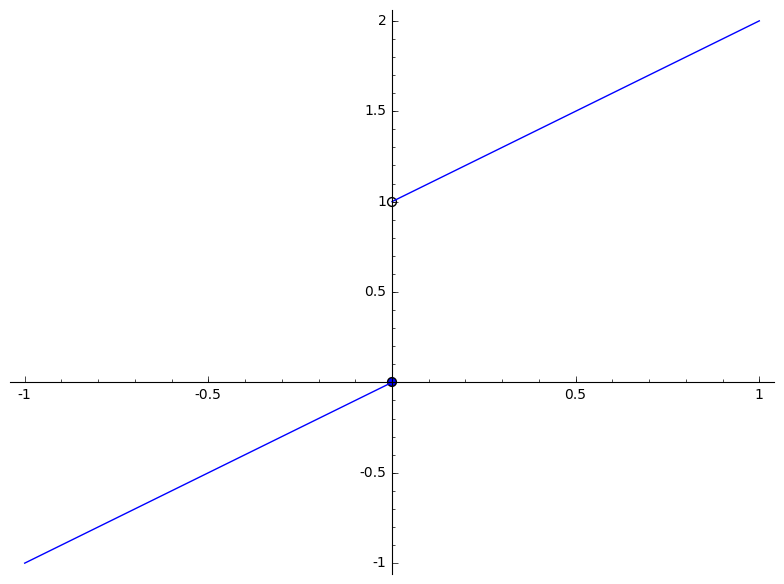
\includegraphics[scale=0.25]{jumpDisc}
      \end{center}
    \end{minipage}}
  \end{multicols}
\end{frame}

\begin{frame}{Removable Discontinuity}
  These usually arise from rational functions:
  \begin{multicols}{2}
    \onslide<2->{\begin{minipage}[t]{0.5\textwidth}
      $$f(x) = \frac{x^2 - 9}{x - 3}$$
    \end{minipage}}
    \columnbreak
    \onslide<3->{
    \begin{minipage}[t]{0.5\textwidth}
      \begin{center}
        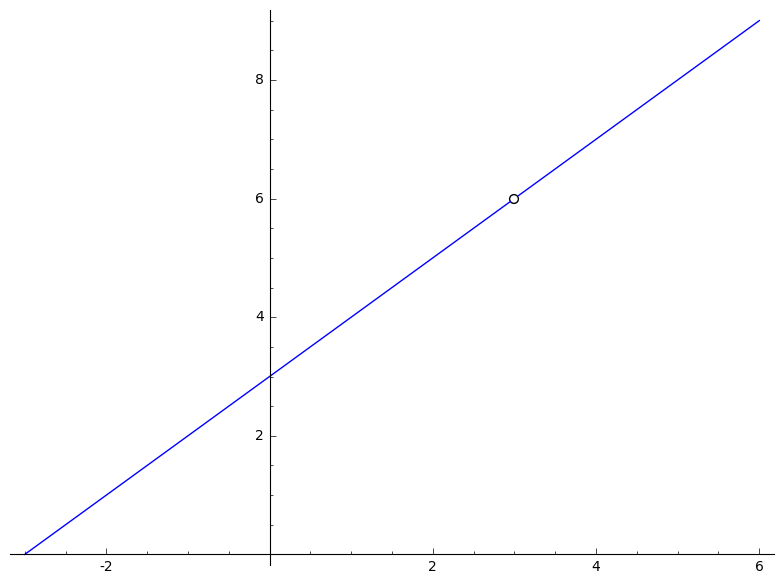
\includegraphics[scale=0.25]{removableDisc}
      \end{center}
    \end{minipage}}
  \end{multicols}
\end{frame}

\begin{frame}{Essential Discontinuity}
  These are discontinuities that cannot be removed by filling in a hole, such as the discontinuity at $x = 0$ of 
  \begin{multicols}{2}
    \onslide<2->{\begin{minipage}[t]{0.5\textwidth}
      $$f(x) = \frac{1}{x}$$
    \end{minipage}}
    \columnbreak
    \onslide<3->{
    \begin{minipage}[t]{0.5\textwidth}
      \begin{center}
        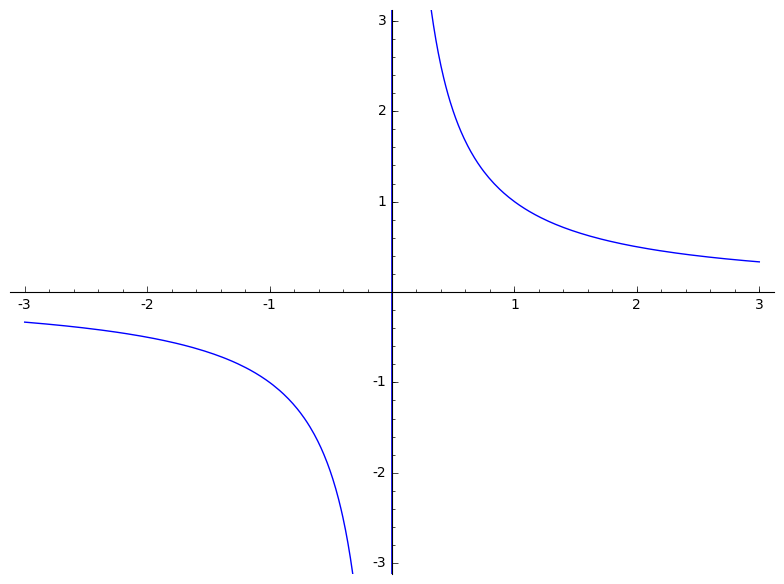
\includegraphics[scale=0.25]{essentialDisc}
      \end{center}
    \end{minipage}}
  \end{multicols}
\end{frame}

\end{document}
